\documentclass[12pt, fullpage,letterpaper]{article}
\usepackage[margin=1in]{geometry}
\usepackage{graphicx}
\title{CS6630 Visualization Fall 2017 Project \\ A Mirror of History}
\author{Yanqing Peng, Yuwei Wang}
\begin{document}
\maketitle
The title \textbf{A mirror of history} comes from the epitaph of Wei Zhen,
a famous Chinese historian:

\emph{``Using copper as a mirror allows one to keep his clothes neat. Using
history as a mirror allows one to see the future trends. Using a person as a
mirror allows one to see what is right and what is wrong.''}

\section{Basic Information}
\paragraph{Title} A Mirror of History
\paragraph{Group members}
\begin{itemize}
    \item Yanqing Peng, u1076076, yq.peng@utah.edu
    \item Yuwei Wang, u1140944, yuwei.utah@gmail.com
\end{itemize}
\paragraph{Github link} https://github.com/uvril/VisProject

\section{Background and Motivation}

History is always fascinating.  It's important to learn lessons from the past,
by understanding the causality behind historical events.  To learn about
history is to learn about humanity, which basically means developing an
understanding of ourselves.  Therefore, knowledge of history helps us prepare
better for future.

However, it can be boring to learn history by texts and numbers. We can know
from textbook that the British Empire used to rule 35,500,000 km$^2$ area of
land. But how large is it?  Showing a map of British Empire is much more
interesting than just telling the number.  Similarly, we know that the economy
of both Japan and Singapore grow dramatically after World War II, but both slow
down in 1990s.  How can we present a comparison between the economy development
of Japan and Singapore?  Showing the GDP table will be boring and hard to
understand.  Instead, showing a line chart for the GDP of Japan and Singapore
is much clearer. Therefore, visualization is essential for learning history.

Our textbooks already contain plenty of figures to visualize history. However,
it's not enough. While learning history, people have different focuses.  Alice
is interested in the border of British Empire in 1913, while Bob wants to see a
map of French colonies in 1908. Charlie would like to know the comparison
between Japan and Singapore, while Eve is curious about the comparison between
India and Pakistan.  Only with interactive visualizations can one develop the
knowledge of history with her own interests.

The course project of CS6630 gives us a golden opportunity to learn better
about history.  In this project, we made a deeper insight into history, by
constructing an interactive visualization on history. We are very happy to see
that we successfully achieve our objectives by using what we've learned from this course.

\section{Related Work}
Chronas

\section{Visualization Objectives}
The main objective of this project is to interactively visualize the current situation of the world,
as well as the historical rise and fall. Our visualization is able to show the following results:

\begin{itemize}

    \item Show the historical world map at a specified year.

    \item Show the basic information (e.g. capital) of a country.

    \item Show the national power of a country in different aspects.

    \item Show the religion in different countries.

    \item Show the ranking of some statistics of a country.

    \item Show the population/gdp/religion distribution of the world.

    \item Show the historical statistics of a country.

    \item Compare the historical statistics of a set of countries.

    \item Show how historical events related to the historical statistics.

\end{itemize}

\section{Data and Resources}
In our project, we use a very wide range of data and resources. We spent a lot of time on data collection and processing.
    In our project, all data are processed into json format. Different catagories
    of data are stored in different files. For example, "pop.json" store all population data.
    If the data file is a historical dataset, then the year attribute is the root attribute, and the country ID is the secondary attribute.
    Otherwise, the country ID is the root attribute.
In this section, we describe the sources of the data, and how we process the data.
\subsection{Country Indexing}
    A major challenge we encountered when processing the data is the issue of country indexing. Our dataset contains 
    formal countries that no longer exist, so we can't use any modern country code to index the countries.
    Moreover, there are countries that have alternative names. For example, "South Korea" and "Republic of Korea" are the same,
    but they are used interchangably in different datasets.
    We have to insure that they point to the same identifier.

    Finally, we decide to use the Wikidata id as the country index. It can uniquely represent any item that appers in wikipedia.
    Moreover, it helps us to retrieve data from wikidata. In our project, the Capital of a country and Head of State of a country are retrieved by wikidata.

    We can use Wikidata queries to convert a country name to its Wikidata ID, using the following query:

        \begin{verbatim}
        SELECT ?child ?childLabel
        WHERE {
              ?child wdt:P31 wd:Q6256.
              ?child  rdfs:label ?childLabel.
              filter (lang(?childLabel) = "en").
              filter (contains(?childLabel, "COUNTRYNAME")).
        }
        \end{verbatim}

        Figure \ref{} illustrates an example for looking up the wikidata id for United States. From the result we can see that the wikidata id for United States is 30.
        However, for some countries that have alternative names, we have to manually build the mapping for them.

        The converted mapping is stored in \textbf{data/wd.csv}.

        For non-historical dataset, most of them contains an ISO 3166 country code field to help identify the countries. With the country code,
        we can easily convert them to wikidata id using the following query:

        \begin{verbatim}
        SELECT ?name WHERE {
        ?name wdt:P298 "COUNTRYCODE".
        }
        \end{verbatim}
        Figure \ref{} illustrates an example for looking up the wikidata id for country with country code "DZA".
        With the country code, we don't need to worry about the alternative name things. However, as explained above,
        it works only for non-historical dataset.
        
        The converted mapping is stored in \textbf{data/cc.csv}.

\subsection{GeoJSON Map Data}
    We collect the GeoJson map data from www.thenmap.net.
    It provides world maps after World War II.
        Although this website doesn't provide the off-the-shelf dataset, one of its
        APIs supports querying for the world map at a specific year. The API
        we used looks like following:

        \begin{verbatim}
        wget http://api.thenmap.net/v1/world-2/geo|data/1946?data_props=name|wikidata
        \end{verbatim}

        This query retrieves the world map at 1946 with the metadata of country name as well as
        the wikidata id for the country. The wikidata ID is essential for future data collection
        such as population.

        Therefore, we wrote a script to automatically download all map data
        from 1946 to 2017 from the website.  To save space, we further did a
        comparison between data of consecutive years, and remove the latter
        data if the world map doesn't change.

        The download script is \textbf{data\_collection/download.py}.
        
        The comparison script is \textbf{data\_collection/remove\_dup.py}.

\subsection{National Flag Icon Resource}

    We use the national flag icons from https://vathanx.deviantart.com/.
    The origional icons are of name "flag\_of\_COUNTRYNAME". We use data/wd.csv
    to convert them into names "WIKIDATAID.ico". These icons are stored in folder \textbf{icons/}.


\subsection{Statistics Data}
    The statistics data are retrieved from wikidata. Since we use the Wikidata ID as the unique ID of countries,
    retrieving information from wikidata can be very easy.

\subsection{Population, GDP, CPI Historical Data}
    s
\subsection{National Power Radar Plot Data}
    The National Power Radar use five datasets: GDP for economy, HDI for
    development, EIU for democracy, EPI for environment, and GFP for military.
    Since these datasets have different domains, we scale all data into range
    $[0,100]$ before plotting them on the screen.

    The radar plot dataset is stored in \textbf{data/radar.json}.

\subsection{Religion Data}
    http://www.thearda.com/Archive/Files/Descriptions/WRDNATL.asp

    The original dataset provides very detailed catagory. To simplify visualization,
    we only use a coarse granularity of catagory (say, Christianity), instead of detailed catagories (say, Catholics).

\section{Design Evolution}
    \subsection{Dataset Change}
        In our proposal and Milestone, we use a dataset contains ancient data (as early as 2000 BC.).
        In our final design, however, we only use dataset since 1960.
        This is mainly because the statistics for ancient countries are largely missing.
        Especially for modern indexes like Human Development Index (HDI), obviously we are not able to get the corresponding data for ancient countries.
        In order to make our visualization consist, we made the hard decision to use only recent data.

    \subsection{Visualization Change}
        Our original design is shown in Figure \ref{}. However, when implementing it, we realized that there were a lot of issues in this design.

        The major issue is that we underestimed the spaced needed for world map. Since we are showing a world map and wish that
        each country is selectable, the map requires a very large space. Figure \ref{} shows the original design. We can see that it's very hard to select a desired country, even with zooming.
        Therefore, we deside to use the whole screen for world map, and reorganize other panels either aggregated in map or create a new tab for them.

        Besides, we find that if we just list the statistics like GDP as Figure \ref{}, these information overlap with the information in the comparison panel.
        Therefore, we adopted a different visualization: we now use a radar chart to represent an overview of national power in different aspects,
        and a donut chart to show the religion in the country. In other words, visualizations in information panels are supposed to be fancy and highly intuitive,
        and those in comparison panel should be formal, accurate and detailed.
\newpage

\section{Implementation}

\paragraph{Get started!} (Nov 4)

After spending a lot of time on data collecting, we successfully collected
the raw data of the historical country borders. The data we collected come
from two different data sets:

\begin{itemize}
    \item For maps after World War II (1946-2017), we collect from www.thenmap.net.
        Although this website doesn't provide the off-the-shelf dataset, one of its
        APIs supports querying for the world map at a specific year after WW2. The API
        we used looks like following:

        \begin{verbatim}
        wget http://api.thenmap.net/v1/world-2/geo|data/1946?data_props=name|wikidata
        \end{verbatim}

        This query retrieves the world map at 1946 with the metadata of country name as well as
        the wikidata id for the country. The wikidata ID is essential for future data collection
        such as population.

    \item For maps from 2000BC to 1945, we find the dataset in a cartography forum (http://www.cartotalk.com/index.php?showtopic=3462).
        The author is anonymous.
        The dataset only contains a few years. That's reasonable enouth -- we never expect to
        find a dataset contains all data from 2000BC to 2017AD!

\end{itemize}

For other data (e.g. population), it seems promising to retrieve them from Wikidata.
We plan to explore the possibility for that.
The first dataset already includes the Wikidata ID for all countries.
We may have to do some data processing on the second dataset to add the Wikidata ID information to it.

\newpage
\paragraph{Implementing the map} (Nov 5)

We implemented a prototype of the map chart and the year chart.
It looks like the follwing (Figure \ref{fig:nov5}):

\begin{figure}[h!]
    \begin{center}
        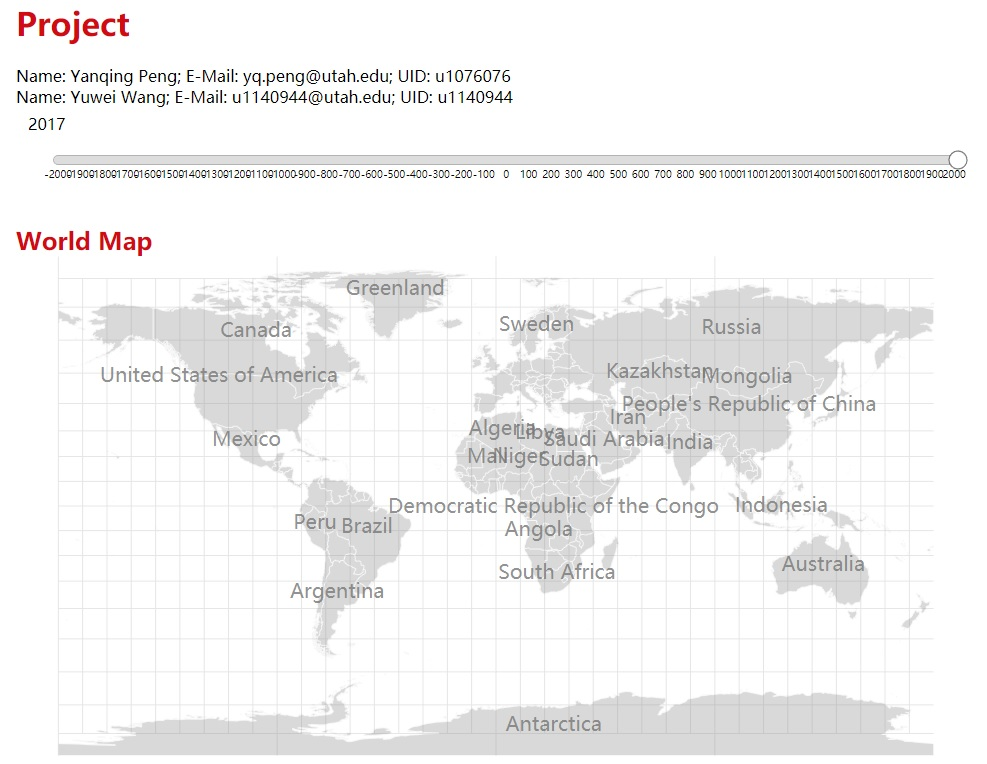
\includegraphics[width=0.9\textwidth]{figs/Nov5.jpg}
        \caption{Current state of our project, Nov 5.}
        \label{fig:nov5}
    \end{center}
\end{figure}

For the year chart, there is a slide bar and a circle which we can drag to choose the desired year.
When the choice of year is updated, the map chart read the dataset with the nearest year before the selected year,
and draw it on the screen. The projection we currently use is d3.geoPatterson().

Adding label is quite challenging. If we simply put all labels on the map,
then there will be a mess in Europe. Currently we only show the labels for countries
with areas larger than a threshold. That doesn't work for countries with large area but extremely
long names (e.g. Democratic Republic of the Congo). Whether or not a label is shown
should depend on both country area and the length of country name. We should think carefully about it.

The location of the labels is another issue. Currently we put the label
at the centroid of the corresponding path. But it doesn't work for some countries like the U.S.
The label of U.S. is actually located inside Canada because of Alaska.
We have to find a smarter way to locate the labels.

\newpage
\paragraph{Layout design, and more on label placement} (Nov 6)

We finished a prototype of the info panel. We also improved the label placement.
As shown in Figure \ref{fig:nov6}, now it looks better, isn't it?

\begin{figure}[h!]
    \begin{center}
        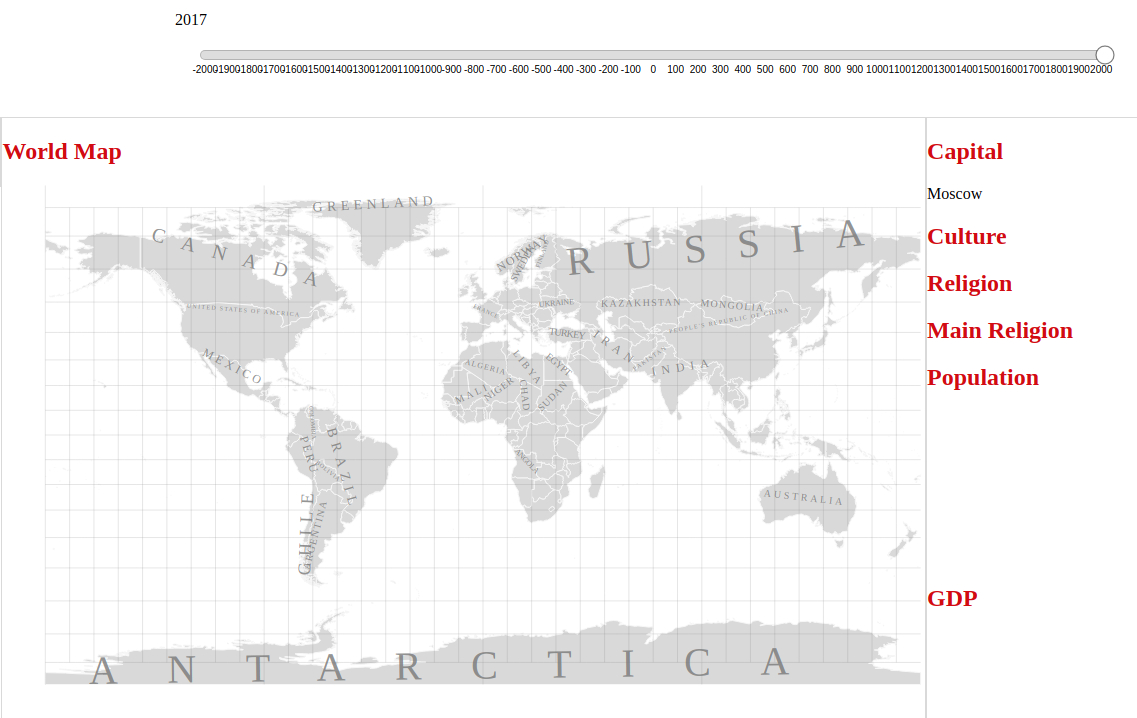
\includegraphics[width=0.8\textwidth]{figs/Nov6.png}
        \caption{Current state of our project, Nov 6.}
        \label{fig:nov6}
    \end{center}
\end{figure}

As shown in the above figure, the information of the capital of a given country
has already been successfully shown. We use Wikidata to retrieve all such information.
The query uses SPARQL. As an example, if we want to know the current capital of Russia,
the language looks like the following:

\begin{verbatim}
SELECT ?name WHERE {
            wd:Q159 wdt:P36 ?link.
            ?link rdfs:label ?name.
            filter (lang(?name) = "en").
}
\end{verbatim}

Where wd:Q159 is the wikidata id of Russia, wdt:P36 is the wikidata id of the property ``capital is'',
and the variable ?link becomes the capital of Russia. Note that ?link itself is also a wikidata id,
which is Q649 in this case. We want to know what Q649 is, so we use the second line in the where clause to retrieve
the its label, and use the third line to restrict the answer to be in English.

For the label placement, we devised a smarter way to put the labels. We first decompose
each country into continous polygons, and pick the polygon with largest area (e.g. for the U.S., only the continent part will remain).
Then we calculated the longest segment within the polygon, and place the label on that line.
The font size will be dynamically adjusted according to the ratio between the segment length and the label length.


\newpage
\paragraph{Information retrieval ready} (Nov 7)

We finished most information retrieval part, as well as the css style for selected country.
We also did a little improvement on label placing:
instead of just placing the text on the diameter of the polygon, now the text is placed on a curve
going from one end of the diameter to the centroid, then to the other end of the diameter.
As shown in Figure \ref{fig:nov7}, it significantly improve the effect for countries with trapezoidal shapes such as U.S. and China, compared
to Figure \ref{fig:nov6}.

\begin{figure}[h!]
    \begin{center}
        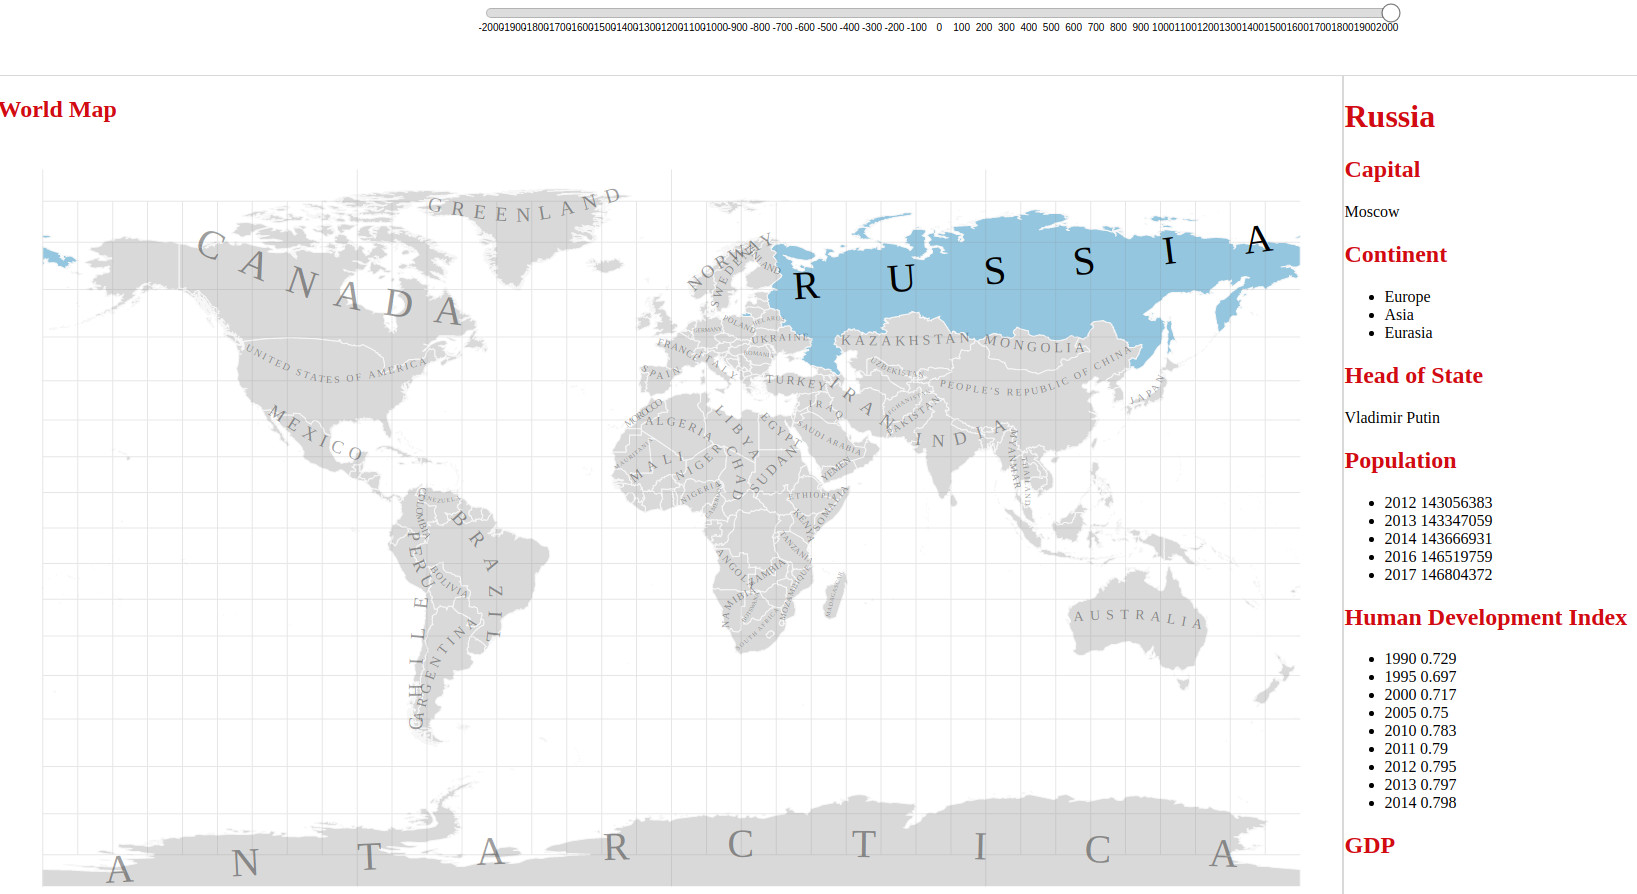
\includegraphics[width=\textwidth]{figs/Nov7.jpg}
        \caption{Current state of our project, Nov 7.}
        \label{fig:nov7}
    \end{center}
\end{figure}

\newpage
\paragraph{InfoPanel design} (Nov 8)

For info panel, currently there are eight parts including selected country name, capital, continents the country belongs to, head of state, population, human development index, territory and description from Wiki.
We retrieved all the data from Wikidata and just put them as original way without any vitualization.
In this way, we found that some data are redundant so deduplicating is necessary.
For example, the continents Russia belongs to include Europe, Asia and Eurasia but Eurasia means Europe and Asia.
In addtion, we decided to label each tile when the mouse hovoring over it since the population data are quite sparse in some areas.

For the description from Wiki, we first tried to bind the source of link with the direct search result from Wikidata.
However, in this way irrelevant infomation takes too much space like the nav bar of Wikipedia. 
We took into account the limitation of the page size and got rid of these infomation by adding "printable=yes" at the end of the link.

\newpage
\paragraph{Visualizing the InfoPanel design} (Nov 10)

We were busy these days. The only progress we made in these days is that we tried to visualize the data
in the information panel. As shown in Figure \ref{fig:nov10}, now the population is shown as a line chart,
and the HDI is shown as a tile chart.

\begin{figure}[h!]
    \begin{center}
        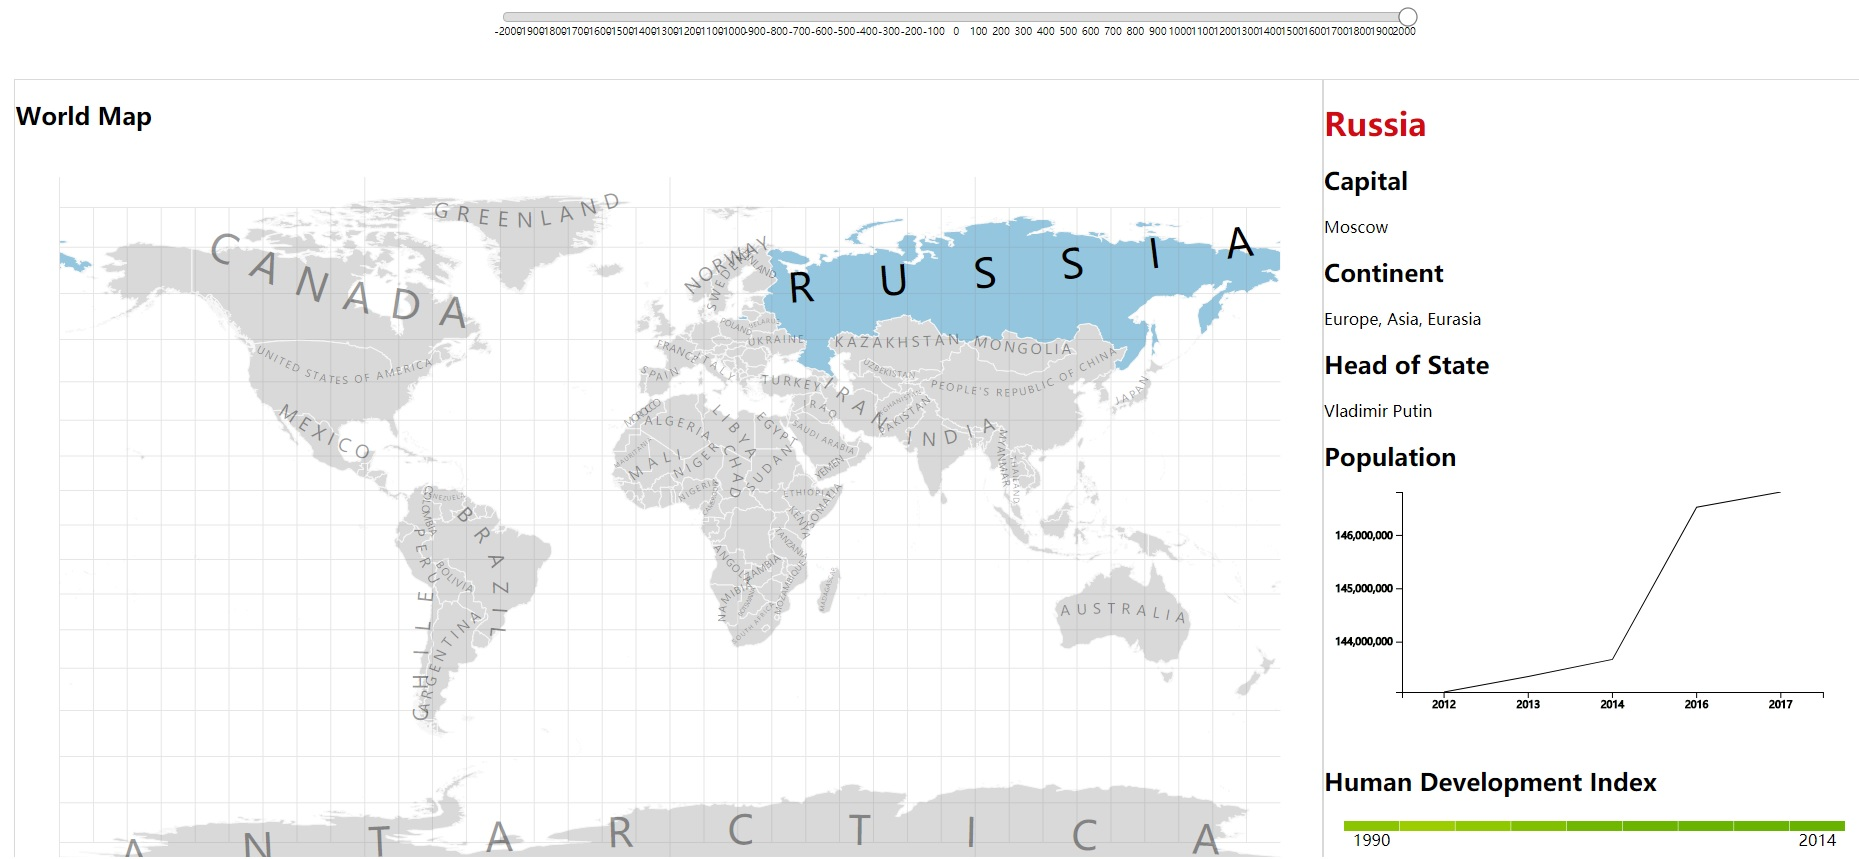
\includegraphics[width=\textwidth]{figs/Nov10.jpg}
        \caption{Current state of our project, Nov 10.}
        \label{fig:nov10}
    \end{center}
\end{figure}

\end{document}
